\chapter{Анализ теоретических основ распознавания многокомпонентных структур и~место задачи реидентификации}\label{ch:ch1}

В~эпоху, когда цифровые технологии становятся неотъемлемой частью многих
сфер жизни общества, фундаментальной задачей информационно-поисковых систем
(ИПС) становится автоматическое распознавание объектов со~сложной
многокомпонентной структурой по~их разрозненным частям. К~этому классу
задач относятся реидентификация человека по~силуэту и~лицу, контроль
технического состояния промышленных конструкций по~локальным дефектам,
идентификация транспортных средств по~номеру и~габаритам, мониторинг
малоразмерных объектов с~борта беспилотных летательных аппаратов и~др.
В~настоящей работе наиболее представительным частным случаем выбрана
задача реидентификации человека: она объединяет в~одной постановке
высокоинформативную, но~часто недоступную модальность лица и~устойчиво
наблюдаемую, но~менее различительную модальность силуэта, требует работы
в~режиме, близком к~реальному времени, и~допускает строгую количественную
оценку на~больших открытых наборах данных. Поэтому в~настоящей главе
изложение строится в~следующей логике: сначала рассматриваются методы
анализа лицевой модальности (\S\ref{sec:ch1/face}) и~методы реидентификации
человека (\S\ref{sec:ch1/reid}), формирующие предметную опору; затем
выполняется обзор коммерческих систем (\S\ref{sec:ch1/commercial}),
а~в~разделе~\S\ref{sec:ch1/math} формализуется общая математическая
постановка задачи распознавания многокомпонентной структуры
с~последующей конкретизацией для $K=2$ (силуэт-лицо). Прогресс в~указанной
области не~только улучшает точность и~эффективность идентификации, но~и~создает
основу для повышения качества широкого класса прикладных ИПС, работающих
в~условиях информационной неопределенности.

\section{Методы и~алгоритмы распознавания человека по~лицу}\label{sec:ch1/face}

Распознавание лиц является одной из~задач в~области распознавания
визуальных образов. Люди постоянно анализируют визуальные образы, получая
информацию через глаза, которую мозг интерпретирует как значимые концепции.
Для компьютера, будь то изображение или видео, это представляет собой
матрицу из~множества пикселей. Задача машины~--- определить, какой концепт
представляет собой определенная часть данных. Это общая проблема
классификации в~распознавании визуальных моделей. В~распознавании лиц
нужно установить, кому принадлежит лицо в~той части данных, которую
машины воспринимают как лицо. Это специализированная задача. В~широком
смысле распознавание лиц включает в~себя связанные технологии для создания
системы распознавания лиц. Оно охватывает обнаружение лиц, определение
положения лица, распознавание личности, предварительную обработку
изображений и~т.\,д. Алгоритм обнаружения лиц заключается в~определении
координат всех лиц на~изображении. Это процесс сканирования всего
изображения для определения, является~ли кандидатская область лицом.
Вывод системы координат лица может быть квадратным, прямоугольным
и~т.\,д. Положение лица~--- это координаты особенностей лица в~системе
координат обнаружения лица. Современные технологии позиционирования
в~основном реализуются с~помощью фреймворков глубокого обучения.
По~сравнению с~обнаружением лиц, время вычислений для алгоритма
позиционирования лица значительно короче. Технология распознавания лиц
основывается на~последовательности шагов, которые преобразуют исходное
изображение в~конкретные данные, позволяющие идентифицировать или
верифицировать человека.

На~первом этапе собираются исходные изображения лиц. Эти изображения
могут быть получены с~камер видеонаблюдения, фотографий или видеопотока.
Предобработка включает в~себя такие операции, как нормализация размера,
коррекция освещенности и~контрастности. Это можно выразить как функцию
предобработки~$P$:
\begin{equation}\label{eq:ch1/preprocess}
    I_{\text{pp}}=P(I_{\text{raw}}),
\end{equation}
где $I_{\text{raw}}$~--- исходное изображение, $I_{\text{pp}}$~---
предобработанное изображение.

После локализации лица на~изображении следующим шагом является извлечение
характерных признаков лица, в~частности контуров глаз, носа, рта и~формы
лица. Процесс может быть представлен как функция~$F$:
\begin{equation}\label{eq:ch1/featext}
    \mathbf{f}_{\text{face}}=F(L),
\end{equation}
где $\mathbf{f}_{\text{face}}$~--- набор признаков лица, извлеченных
из~локализованного изображения лица~$L$.

Извлеченные признаки сравниваются с~данными в~базе для идентификации
или верификации личности. Этот процесс представим как функцию
сопоставления~$M$:
\begin{equation}\label{eq:ch1/match}
    R=M(\mathbf{f}_{\text{face}},\mathrm{DB}),
\end{equation}
где $R$~--- результат сопоставления, $\mathrm{DB}$~--- база данных
признаков лиц.

На~основе результатов сопоставления принимается решение о~том,
соответствует~ли обнаруженное лицо какой-либо записи в~базе данных.
Этот шаг выражается как функция верификации (идентификации)~$V$:
\begin{equation}\label{eq:ch1/verify}
    \mathrm{ID}=V(R),
\end{equation}
где $\mathrm{ID}$~--- идентификатор лица или подтверждение его
соответствия записи в~базе данных.

Эти шаги составляют основу процесса распознавания лиц. Чтобы более
глубоко погрузиться в~область технологий распознавания лиц, необходимо
тщательно рассмотреть ряд научных работ и~исследований, проведенных
в~этой области. Важно ознакомиться с~различными методами и~алгоритмами,
использованными для распознавания лиц, начиная от~традиционных подходов
(HAAR Cascade) и~до современных техник глубокого обучения и~нейронных
сетей. Особое внимание следует уделить исследованиям, касающимся
извлечения и~анализа признаков лица, методов сопоставления и~сравнения
признаков, а~также улучшения точности и~надежности систем распознавания.
Кроме того, важно рассмотреть вопросы, связанные с~эффективностью работы
алгоритмов в~различных условиях: изменение освещения, разные ракурсы
лица и~динамика выражений. Изучение указанных работ дает комплексное
представление о~текущем состоянии технологии, ее ограничениях
и~потенциале для будущих улучшений.

В~области распознавания лиц два метода, не~связанных с~глубоким
обучением,~--- это анализ главных компонент (PCA) и~линейный
дискриминантный анализ (LDA).

Анализ главных компонент (PCA) считается одним из~самых популярных
методов уменьшения размерности данных. В~контексте алгоритмов
распознавания лиц PCA используется для извлечения особенностей лица.
Этот метод был введен в~область распознавания лиц в~1991~году Турком
и~Пентлендом из~Медиа Лаборатории Массачусетского технологического
института (MIT)~\cite{Chen2022keypoint}. Основная цель PCA~--- устранить
избыточную информацию и~шум из~данных, сохраняя при этом их ключевые
характеристики, существенно сокращая размерность данных, ускоряя их
обработку и~экономя время и~ресурсы. Классическим примером алгоритма
на~основе PCA является алгоритм <<eigenface>>~\cite{Gottumukkal2004modularpca,Li2009facePCALDA}.

Линейный дискриминантный анализ (LDA) используется для классификации лиц
в~наборах данных, где имеются метки классов~\cite{Lu2003faceLDA}.
В~отличие от~PCA, который стремится максимизировать дисперсию данных
после сокращения размерности, LDA направлен на~минимизацию
внутриклассовой дисперсии и~максимизацию межклассовой дисперсии. Это
означает, что LDA является методом с~учителем для уменьшения
размерности, использующим информацию о~метках для максимального
разделения различных категорий данных.

Оба метода, PCA и~LDA, являются важными в~классическом распознавании лиц
и~лежат в~основе многих современных методов, основанных на~глубоком
обучении. Они представляют собой фундаментальные подходы в~обработке
изображений и~распознавании лиц до~эры глубокого обучения.

В~работе~\cite{Karthick2021attendance} использовался алгоритм HAAR
Cascade для распознавания лиц, а~также статистические классификаторы
данных~--- анализ главных компонент (PCA) и~линейный дискриминантный
анализ (LDA)~--- для создания методов распознавания лиц.
В~эксперименте были проведены сравнительные тесты и~сделан вывод, что
оба метода имеют одинаковую точность~98\%, что является лучшим
результатом для классификации и~распознавания лиц.

В~работе~\cite{Saranya2020surveillance} было предложено использовать
компьютерное зрение в~системах видеонаблюдения для распознавания лиц
в~реальном времени. Эксперимент был реализован на~оборудовании
Raspberry~Pi~3 с~применением алгоритма Виолы-Джонса и~функции гистограммы
направленных градиентов (HOG) для извлечения черт лица с~помощью
глубокого обучения. Результат эксперимента, основанный на~глубоком
обучении, показал хорошую точность в~идентификации лиц и~последующем
распознавании людей через видеопоток.

\section{Методы реидентификации человека}\label{sec:ch1/reid}

В~эпоху строительства <<умных>> городов по~всему миру устанавливается
большое количество высококачественных камер видеонаблюдения, которые
генерируют многочисленные видеоматериалы. Анализ и~использование данных
о~пешеходах становятся практически значимой задачей. Эти данные
не~только помогают правоохранительным органам быстро находить подсказки
о~подозреваемых или пропавших детях и~пожилых людях, но~и~позволяют
предпринимателям извлекать закономерности поведения пешеходов для более
рационального использования коммерческих ресурсов. Реидентификация
личности~\cite{Wang2020reidoverview} возникает как необходимость времени
и~является ключевой технологией в~создании интеллектуальных систем
наблюдения. Эта технология находит применение во~многих практических
сценариях, в~частности в~статистике движения людей, обнаружении уличных
событий и~анализе поведения личности. Реидентификация
человека~\cite{Wang2020reidoverview} подразумевает использование
технологий компьютерного зрения для определения личности конкретного
человека в~системе мониторинга с~использованием множества
непересекающихся камер. Ставя интересующий запрос, задача
реидентификации человека заключается в~поиске других изображений или
видеопоследовательностей из~коллекции, собранной мультикамерной
системой, и~определении, кто является этим человеком, как показано
на~рис.~\ref{fig:ch1/reid-scheme}.

\begin{figure}[htbp]
\centering
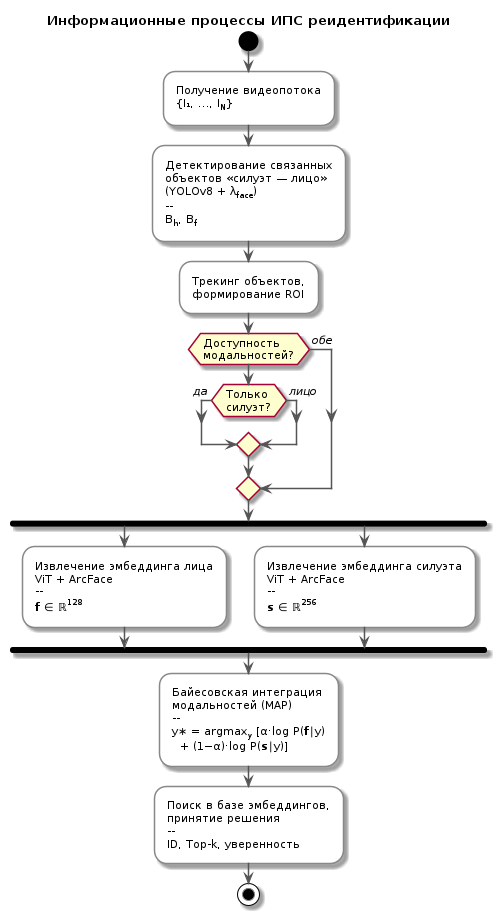
\includegraphics[width=0.85\textwidth,keepaspectratio]{images/1.png}
\caption{Типовая схема системы реидентификации человека (частный случай
многокомпонентной структуры при~$K=2$)}
\label{fig:ch1/reid-scheme}
\end{figure}

Обобщенная схема информационных процессов ИПС для распознавания
многокомпонентной структуры с~произвольным числом компонентов~$K$
приведена на~рис.~\ref{fig:ch1/ipc-generic}. В~ней детектор формирует
ROI всех компонентов структуры, специализированные кодировщики
$\Phi_1,\ldots,\Phi_K$ независимо извлекают признаковые описания, а~их
последующая байесовская интеграция с~MAP-критерием формирует итоговое
решение, согласованное с~текущим набором доступных компонентов
$\mathcal{M}(t)\subseteq\{1,\ldots,K\}$. Рассматриваемая в~работе задача
реидентификации человека по~паре <<силуэт-лицо>> соответствует этой
схеме при~$K=2$.

\begin{figure}[htbp]
\centering
% Обобщённая схема информационных процессов ИПС
% Многокомпонентная структура с K компонентов
\begin{tikzpicture}[
    node distance=4mm and 6mm,
    every node/.style={font=\small},
    block/.style={
        draw, rounded corners, align=center,
        minimum height=8mm, minimum width=24mm,
        inner sep=2pt
    },
    enc/.style={
        draw, align=center,
        minimum height=8mm, minimum width=16mm,
        inner sep=2pt
    },
    bayes/.style={
        draw, thick, rounded corners, align=center,
        minimum height=10mm, minimum width=58mm,
        inner sep=2pt
    },
    arr/.style={-{Latex[length=2mm]}, thick},
    dots/.style={font=\Large},
]
% Вход
\node[block] (img) {Кадр~$I$ видеопотока};

% Детектор
\node[block, below=of img] (det) {Согласованный детектор\\ компонентов структуры};
\draw[arr] (img) -- (det);

% ROI
\node[block, below=8mm of det, minimum width=66mm] (rois)
    {ROI компонентов: $C_1,\,C_2,\,\ldots,\,C_K$};
\draw[arr] (det) -- (rois);

% Энкодеры
\node[enc, below=8mm of rois.west, anchor=north west, xshift=2mm] (e1) {$\Phi_1$};
\node[enc, right=4mm of e1] (e2) {$\Phi_2$};
\node[dots, right=4mm of e2] (edots) {$\cdots$};
\node[enc, right=4mm of edots] (eK) {$\Phi_K$};

\draw[arr] ([xshift=-22mm]rois.south) -- (e1.north);
\draw[arr] ([xshift=-8mm]rois.south) -- (e2.north);
\draw[arr] ([xshift=14mm]rois.south) -- (eK.north);

% Эмбеддинги
\node[below=4mm of e1] (z1) {$\mathbf{z}_1$};
\node[below=4mm of e2] (z2) {$\mathbf{z}_2$};
\node[dots, below=4mm of edots] (zdots) {$\cdots$};
\node[below=4mm of eK] (zK) {$\mathbf{z}_K$};
\draw[arr] (e1) -- (z1);
\draw[arr] (e2) -- (z2);
\draw[arr] (eK) -- (zK);

% Байес
\node[bayes, below=8mm of zdots, fill=black!5] (bayes) {%
    Байесовская интеграция: $\displaystyle P(y\mid\{\mathbf{z}_k\})\propto P(y)\!\!\prod_{k\in\mathcal{M}(t)}\!\!P(\mathbf{z}_k\mid y)$};
\draw[arr] (z1) -- (bayes.north -| z1);
\draw[arr] (z2) -- (bayes.north -| z2);
\draw[arr] (zK) -- (bayes.north -| zK);

% MAP
\node[block, below=6mm of bayes] (map)
    {MAP-критерий: $y^{*}=\displaystyle\arg\max_{y\in Y}\sum_{k\in\mathcal{M}(t)}\log P(\mathbf{z}_k\mid y)$};
\draw[arr] (bayes) -- (map);

% Решение
\node[block, below=6mm of map] (out) {Решение $y^{*}$};
\draw[arr] (map) -- (out);

\end{tikzpicture}

\caption{Обобщенная схема информационных процессов ИПС для распознавания
многокомпонентной структуры из~$K$ компонентов}
\label{fig:ch1/ipc-generic}
\end{figure}

Концепция реидентификации человека впервые была определена в~2006~году
в~работе~\cite{Gheissari2006reid}. С~тех пор данное направление пережило
быстрое развитие, и~ученые всего мира провели обширные исследования этой
задачи, разработав множество подходов. Однако существующие подходы
многочисленны и~имеют различные акценты. Поэтому, чтобы помочь
исследователям, вступающим в~эту область, быстро ориентироваться в~ее
развитии и~получить обзор перспективных направлений, в~настоящем
разделе изучается поле реидентификации человека и~подводятся итоги
связанных с~ним понятий и~достижений.

В~ряде фундаментальных работ~\cite{Zheng2016reidsurvey,Chahar2017reid,Wu2019reidsurvey}
представлен обзор современных тенденций в~области реидентификации
человека и~анализ крупных наборов данных, а~также методов глубокого
обучения. Однако данные исследования фокусируются преимущественно
на~отдельных аспектах: авторы~\cite{Han2019ghostnet,He2015resnet}
детально рассматривают различные фреймворки и~подходы к~оценке
эффективности, а~также затрагивают задачу реидентификации гетерогенных
личностей, но~в~их обзорах отсутствует углубленная классификация
алгоритмов и~не~уделяется должного внимания широкому спектру методов
(в~частности, переранжированию результатов). В~более ранних работах,
в~частности~\cite{BedagkarGala2014survey}, реидентификация изучалась
до~формирования доминирующей роли глубокого обучения, которое начало
активно развиваться после 2014~года. Это привело к~тому, что
в~обзоре~\cite{BedagkarGala2014survey} часть современных методов
и~достижений, связанных с~применением сверточных нейронных сетей
и~трансформеров, по~понятным причинам не~представлена. В~относительно
недавнем исследовании~\cite{Wu2019reidsurvey} авторы провели детальный
анализ датасетов, функций потерь и~методов реидентификации человека,
однако не~представили логическую классификацию существующих подходов
и~не~рассмотрели целый ряд важных аспектов, в~частности процедуры
переранжирования (re-ranking) результатов и~стратегий на~основе сетей
камер, которые имеют большое практическое значение в~реальных системах
видеонаблюдения. Таким образом, несмотря на~очевидный прогресс
в~области реидентификации, остается потребность в~более целостном
и~структурированном обзоре, который охватил бы не~только современные
алгоритмы глубокого обучения, но~и~их интеграцию в~многоаспектные
системы обработки.

\section{Коммерческие системы распознавания человека}\label{sec:ch1/commercial}

Российский рынок биометрических технологий за~период с~2014 по~2018~год
показал значительный рост. Ежегодный средний прирост в~этот период
составил 35,72\%, что свидетельствует о~быстром развитии и~внедрении
биометрических технологий в~различных секторах~\cite{Nazarova2023biometry}.
На~конец 2018~года объем рынка достиг 5,6~млрд рублей. Этот рост
объясняется как увеличением спроса на~биометрические технологии
со~стороны коммерческих и~государственных организаций, так и~активным
развитием технологий в~этой области. Указанная динамика существенно
выше среднемировых показателей и~подчеркивает растущее значение
биометрических технологий в~России. Это увеличение способствует
дальнейшему развитию и~интеграции биометрических систем во~многие
аспекты общественной жизни, в~частности в~безопасность, финансовые
услуги и~потребительские технологии.

Среди ключевых тенденций рынка выделяются:
\begin{itemize}
    \item снижение ошибок I~и~II рода, увеличение скорости распознавания
          и~сравнения;
    \item удобство использования и~интеграции в~клиентские сервисы
          стимулирует развитие технологий удаленной идентификации;
    \item сочетание биометрии с~небиометрическими данными (например,
          PIN/карта) или использование мультибиометрических систем для
          повышения надежности.
\end{itemize}

На~российском рынке преобладают следующие биометрические технологии:
\begin{itemize}
    \item распознавание отпечатков пальцев, которое широко распространено
          в~системах контроля доступа и~криминалистике, но~уступает
          по~надежности и~скорости идентификации другим технологиям;
    \item васкулярное сканирование, наращивающее долю на~рынке благодаря
          более высокой надежности по~сравнению с~отпечатками пальцев
          и~лицевой биометрией; однако ограничено в~удаленных системах
          идентификации из-за своей <<контактности>>;
    \item распознавание лиц, имеющее преимущества в~простоте и~скорости
          сбора данных, бесконтактности, возможности реализации
          идентификации <<в~потоке>> и~удаленных систем; не~требует
          специализированного оборудования;
    \item распознавание голоса~--- наименее надежная и~уязвимая
          к~изменениям внешних условий технология, остается нишевым
          продуктом;
    \item аутентификация по~радужной оболочке глаза~--- самая надежная
          технология, однако из-за высокой стоимости не~получила
          массового распространения.
\end{itemize}

При этом распознавание лиц занимает наибольшую долю на~российском рынке,
что отличает его от~мирового, где преобладает Fingerprint. В~2018~году
доля этого сегмента составила 49,6\% от~всего рынка. В~отличие
от~мирового рынка, где доминируют <<пальчиковые>> технологии, в~России
развитие шло в~направлении лицевой биометрии. Российские компании стали
одними из~лучших в~мире в~области систем распознавания лиц.

Общий анализ коммерческих систем распознавания человека в~России выявляет
растущую долю систем идентификации людей на~рынке, подкрепленную
технологическими инновациями и~государственной поддержкой. В~то же время
разнообразие доступных технологий показывает динамичность и~адаптивность
рынка к~изменяющимся требованиям безопасности и~идентификации.

\section{Математическая постановка задачи}\label{sec:ch1/math}

В~рамках данного исследования ставится задача создания алгоритмического
комплекса для распознавания и~реидентификации человека на~основе
изображений, полученных из~разнообразных источников. Основная цель~---
разработать набор математических функций и~процедур, которые обеспечивают
точное выделение, анализ и~синтез ключевых признаков человека,
представленного на~изображениях. Это включает в~себя функции
детектирования силуэтов и~лиц, функции преобразования выделенных объектов
в~векторы признаков, а~также разработку методов комбинирования
и~идентификации на~основе этих векторов. Основным вызовом здесь является
не~только точность детектирования и~распознавания, но~и~оптимизация
вычислительных процессов для обработки больших объемов данных.

Дано:
\begin{itemize}
    \item множество изображений
    \begin{equation}\label{eq:ch1/images}
        \mathcal{I}=\{I_i\}_{i=1}^{N_I},
    \end{equation}
    где каждое изображение $I_i$ содержит одного или несколько людей;

    \item функция детектирования силуэта $D_h(\cdot)$, возвращающая
    множество силуэтов $B_h$ для изображения~$I$;

    \item функция детектирования лица $D_f(\cdot)$, возвращающая
    множество лиц $B_f$ для изображения~$I$ или пустое множество, если
    лицо не~обнаружено;

    \item функция извлечения признаков $\Phi(\cdot)$, преобразующая
    детектированный объект (силуэт или лицо) в~вектор в~пространстве
    признаков.
\end{itemize}

Необходимо:
\begin{enumerate}
    \item разработать функцию комбинирования $g(\cdot)$, которая
    принимает на~вход вектор силуэта~$\mathbf{s}$ и~вектор
    лица~$\mathbf{f}$ (если лицо было обнаружено) и~возвращает
    комбинированный вектор признаков~$\mathbf{z}$:
    \begin{equation}\label{eq:ch1/combine}
        \mathbf{z}=g(\mathbf{s},\mathbf{f});
    \end{equation}

    \item разработать функцию идентификации $A(\cdot)$, которая
    принимает на~вход комбинированный вектор признаков~$\mathbf{z}$
    и~базу данных векторов~$\mathrm{DB}$ и~возвращает результат
    идентификации.
\end{enumerate}

\textbf{Задача.} Построить систему, которая, принимая на~вход
изображение~$I$, выполняет следующие шаги:
\begin{enumerate}
    \item детектирование силуэта и~лица на~изображении~$I$
          с~использованием функций $D_h$ и~$D_f$:
    \begin{equation}\label{eq:ch1/detect}
        B_h=D_h(I),\quad B_f=D_f(I);
    \end{equation}

    \item преобразование детектированных объектов в~векторы с~помощью
          функции $\Phi(\cdot)$:
    \begin{equation}\label{eq:ch1/emb-h}
        \mathbf{s}=\Phi(\mathrm{ROI}_{\text{human}}),
    \end{equation}
    \begin{equation}\label{eq:ch1/emb-f}
        \mathbf{f}=\Phi(\mathrm{ROI}_{\text{face}});
    \end{equation}

    \item комбинирование векторов согласно~(\ref{eq:ch1/combine});

    \item идентификацию на~основе комбинированного вектора признаков
          с~использованием функции $A(\cdot)$ по~базе $\mathrm{DB}$.
\end{enumerate}

\textbf{Цель:} минимизировать ошибку идентификации при оптимальных
вычислительных затратах. Это включает в~себя определение оптимальной
структуры и~параметров для функций $D_h$, $D_f$, $\Phi$, $g$ и~$A$,
а~также выбор наиболее подходящих алгоритмов машинного обучения
и~техник оптимизации для достижения поставленной цели.

\section{Выводы по~главе}\label{sec:ch1/conclusion}

В~главе последовательно рассмотрены методы и~алгоритмы, составляющие
полный контур информационно-поисковой обработки видеоданных в~задачах
поиска и~реидентификации человека. Проанализированы современные подходы
к~детектированию человеческих фигур и~лиц, особенности локализации лица
внутри силуэта как критического частного случая, а~также архитектуры
построения признаковых представлений для обеих модальностей. Отдельное
внимание уделено метрикам обучения и~сопоставления, которые определяют
корректность идентификации и~реидентификации, и~стратегиям интеграции
многомодальных признаков. Рассмотрены общепринятые наборы данных
и~процедуры оценки качества, закрепляющие воспроизводимость результатов
и~сопоставимость с~базовыми решениями.

Проведенный анализ существующих решений показал ключевую роль
детектирования как входного фильтра контура. Установлено, что неточности
на~этапе локализации объектов приводят к~каскадному ухудшению качества
на~последующих стадиях, искажают построение эмбеддингов и~снижают
точность сопоставления. Показано, что однофакторные схемы, опирающиеся
исключительно на~лицевые либо исключительно на~силуэтные признаки,
недостаточно устойчивы в~условиях изменчивой сцены: вариации ракурса
и~освещения, окклюзии и~неполная видимость приводят к~росту ложных
тревог и~пропусков. Выявлено, что современные архитектуры для
формирования признаковых представлений обеспечивают более высокую
дискриминативность при соблюдении требований к~регуляризации и~объему
данных, однако их применение должно быть согласовано с~вычислительными
ограничениями системы, ориентированной на~работу в~реальном времени.

Сопоставление подходов позволило зафиксировать их преимущества
и~ограничения. К~достоинствам многофакторных схем относится повышенная
устойчивость к~внешним возмущениям и~способность компенсировать
частичные отказы модальностей, что выражается в~росте интегральных
метрик качества. Вместе с~тем тяжелые модели детектирования
и~эмбеддинга увеличивают задержки и~нагрузку на~вычислительные ресурсы;
фиксированные веса при слиянии модальностей оказываются неадаптивными
к~смене условий съемки, а~каскадный характер контура усиливает влияние
ошибок начального этапа. Таким образом, практическая применимость
решений определяется не~только точностью отдельных алгоритмов, но~и~их
согласованной работой под эксплуатационные метрики
информационно-поисковой системы.

Суммарный анализ выявил методологический разрыв между требованиями
эксплуатации и~свойствами распространенных схем. Для его преодоления
требуется, во-первых, усилить этап детектирования, включая обработку
сценариев вложенного поиска лиц внутри силуэта; во-вторых, обеспечить
построение компактных и~устойчивых признаковых представлений для лица
и~силуэта с~учетом доменных факторов; в-третьих, применять адаптивную
интеграцию модальностей, учитывающую надежность и~доступность
источников признаков в~конкретной сцене; в-четвертых, формулировать
и~оптимизировать целевые функции, напрямую связанные с~эксплуатационными
метриками (mAP, Rank-k, ROC/PR) при соблюдении ограничений по~времени
отклика.

Сформулированные выводы определяют содержание последующих разделов
работы: разработку методики детектирования, ориентированной на~снижение
каскадных ошибок; построение эмбеддингов для обеих модальностей
с~требуемой дискриминативностью и~компактностью; разработку алгоритмов
автоматической настройки ключевых гиперпараметров; реализацию
вероятностной, по~сути байесовской, интеграции признаков, адаптирующей
вклад модальностей к~контексту сцены; а~также экспериментальную
верификацию на~репрезентативных наборах данных с~отчетными метриками
и~анализом уверенности решений. В~совокупности эти элементы создают
основу для последующего повышения точности поиска и~реидентификации
человека при рациональных вычислительных затратах.
